%\textcolor{red}{\textbf{present vs past -- consistency!   ||  what about size of text in figures?}}
\subsection*{Population circadian gene expression is layer-specific in healthy human skin} 
To explore molecular circadian rhythms in human dermis and epidermis, 11 healthy subjects (male and female) were biopsied in the upper back every 4\,h across a 24\,h duration (Figure \ref{fig:fig1}A, Materials and Methods). Subjects were asked to maintain their desired sleep-wake schedule in the 2 weeks leading up to the sampling. Samples were separated into dermis and epidermis and subsequently quantified using whole-genome microarrays. We adjusted sample collection times using their chronotypes to indicate \emph{internal} time of subjects (Figure \ref{fig:fig1}B). Chronotypes were estimated from sleep schedules (\textcolor{red}{available in Supplementary Table \ref{tab:supptab1}}) as the mid-sleep time on free days after correcting for sleep debt ($\textrm{MSF}_\textrm{sc}$) \cite{Vetter2021}. \todo{Better in the MM -- For each subject, internal time was determined by subtracting wall time minus the difference of his/her MST to a reference subject (the individual with median MST).}

A large majority of circadian genes were rhythmic in both layers. We identified and compared genes with circadian population rhythms in both human skin layers using differential rhythmicity analysis \cite{Pelikan2021}. \textit{Population} rhythms are circadian patterns of gene expression averaged across the entire cohort. We identified 1053 circadian genes in dermis and 1352 in epidermis (FDR $<0.05$ and amplitude $>1.5$ fold peak-to-trough), of which 966 genes were rhythmic in both skin layers (Figure \ref{fig:fig1}C, inset, Supplementary Figure \ref{fig:suppfig2}A). The number of circadian genes remained stable across a range of choices of FDR cutoff (Figure \ref{fig:fig1}C). 386 genes were rhythmic only in the epidermis and 87 only in the dermis, as well as a further 49 genes that were rhythmic in both but with significantly different amplitude and/or phase.

\begin{figure*}[b!]
	\begin{center}
		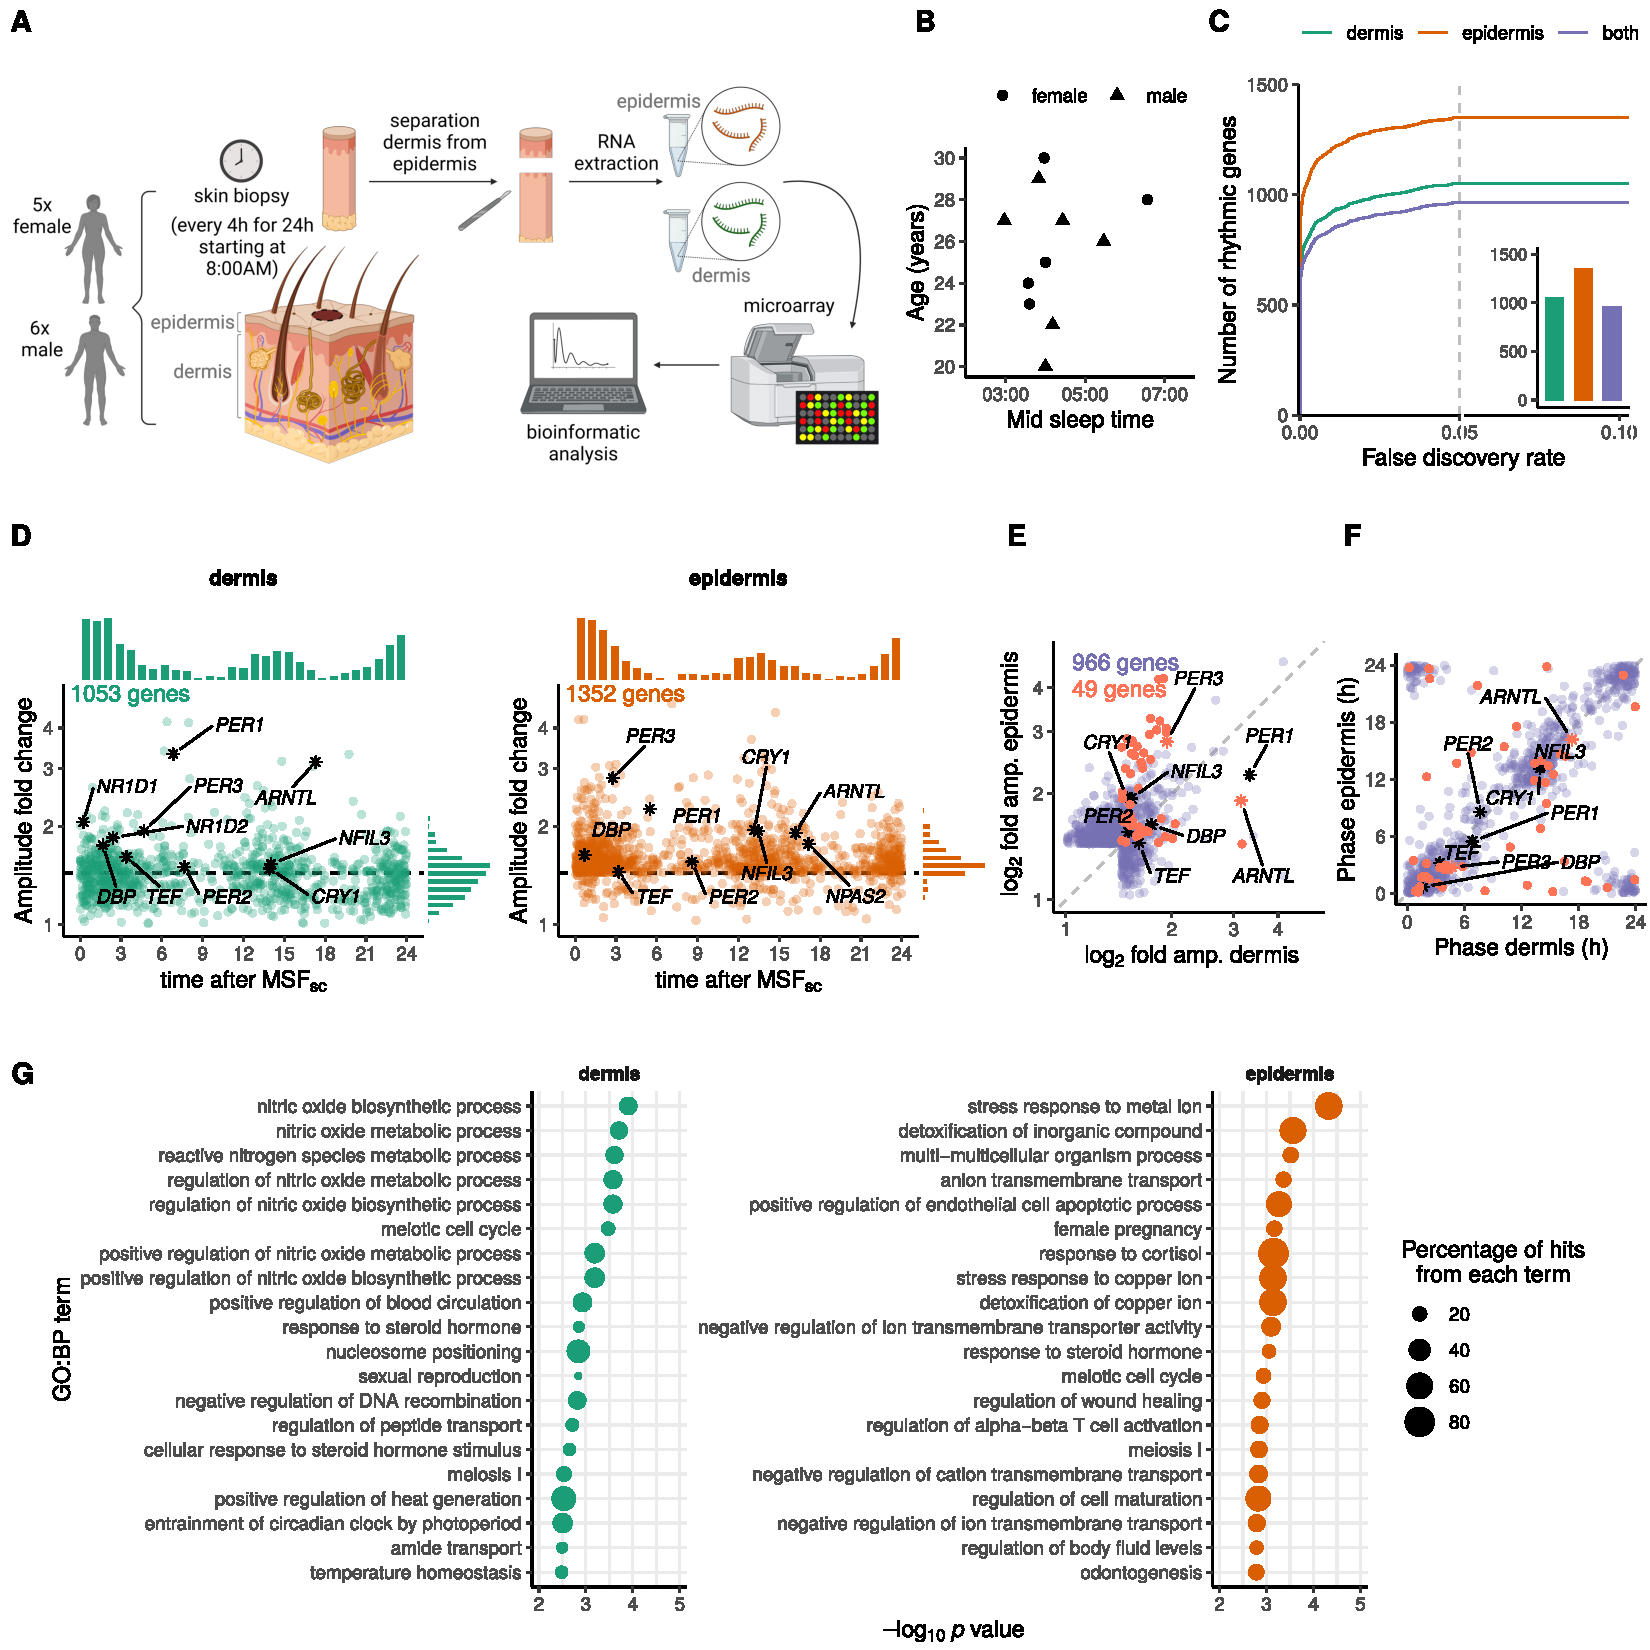
\includegraphics[scale=0.55]{./Figures/fig1_complete.pdf}
		%\caption{\textbf{Functional (and different) clocks in human dermis and epidermis. A.} Experimental setup: the dataset includes dermis and epidermis samples collected from 11 subjects (5 females, 6 males) from the \textcolor{red}{arm}. Skin biopsies were collected every 4\,h for 24\,h starting at 8\,AM. Dermis and epidermis were separated \textcolor{red}{...} and gene expression was analyzed using microarrays.\textbf{ B. }Composition of the study cohort by sex, age and mid sleep time. \textbf{C. }Number of circadian transcripts as a function of the false discovery rate (FDR). Rhythmic transcripts in dermis, epidermis or in both layers were determined by cosinor analysis (\textcolor{red}{FC amplitude$>0.26$}, one single test, in the lines of \cite{Pelikan2021}). Internal time was used for the analysis and was calculated as wall time (i.e., time of sampling) minus the difference in mid sleep time of each subject to a reference subject (that with median mid sleep time). For FDR$=0.05$, 523 transcripts were found to oscillate with a circadian period in dermis, 1191 in epidermis and 283 were common in both layers (bar plots from inset, \textcolor{red}{FC amplitude$>0.26$}). \textbf{D. }Acrophase and amplitude distributions of the 24\,h cycling transcripts in human dermis (in green, left panel) and epidermis (orange, right panel). Each transcript is represented by a dot; clock genes are highlighted in black. Acrophases and amplitudes were estimated from the cosinor analysis at FDR$<0.05$; \textcolor{red}{the minimal FC amplitude for cycling transcripts was set to 0.26}. \textbf{E. }Amplitude correlation of cycling transcripts in dermis \textit{and} epidermis. \textbf{F. }Phase correlation of cycling transcripts in dermis \textit{and} epidermis. \textbf{G.} Circadian GO enrichment analysis of the rhythmic genes in dermis (green) and epidermis (orange). The top 20 enriched biological processes (with a minimum gene set of 5 terms from each category) in each layer are shown. } %Thresholds: transform $\log(1+0.2)$ to ``biological words''.Maybe TODO: use internal time together with amp and phase fits to plot the gene expression curves in all 11 subjects. Then plot mean curve and determine amplitude from the population curve. Do the same but with wall time: Do amplitudes change? For which genes? \textcolor{red}{Think about DOSE with weights -- there was one skin term! Commented at end of 4th paragraph}. mingene set size=5}
%\label{fig:fig1}
	\end{center}
\end{figure*}
\newpage
\begin{figure*}%[htb!]
	\begin{center}
		%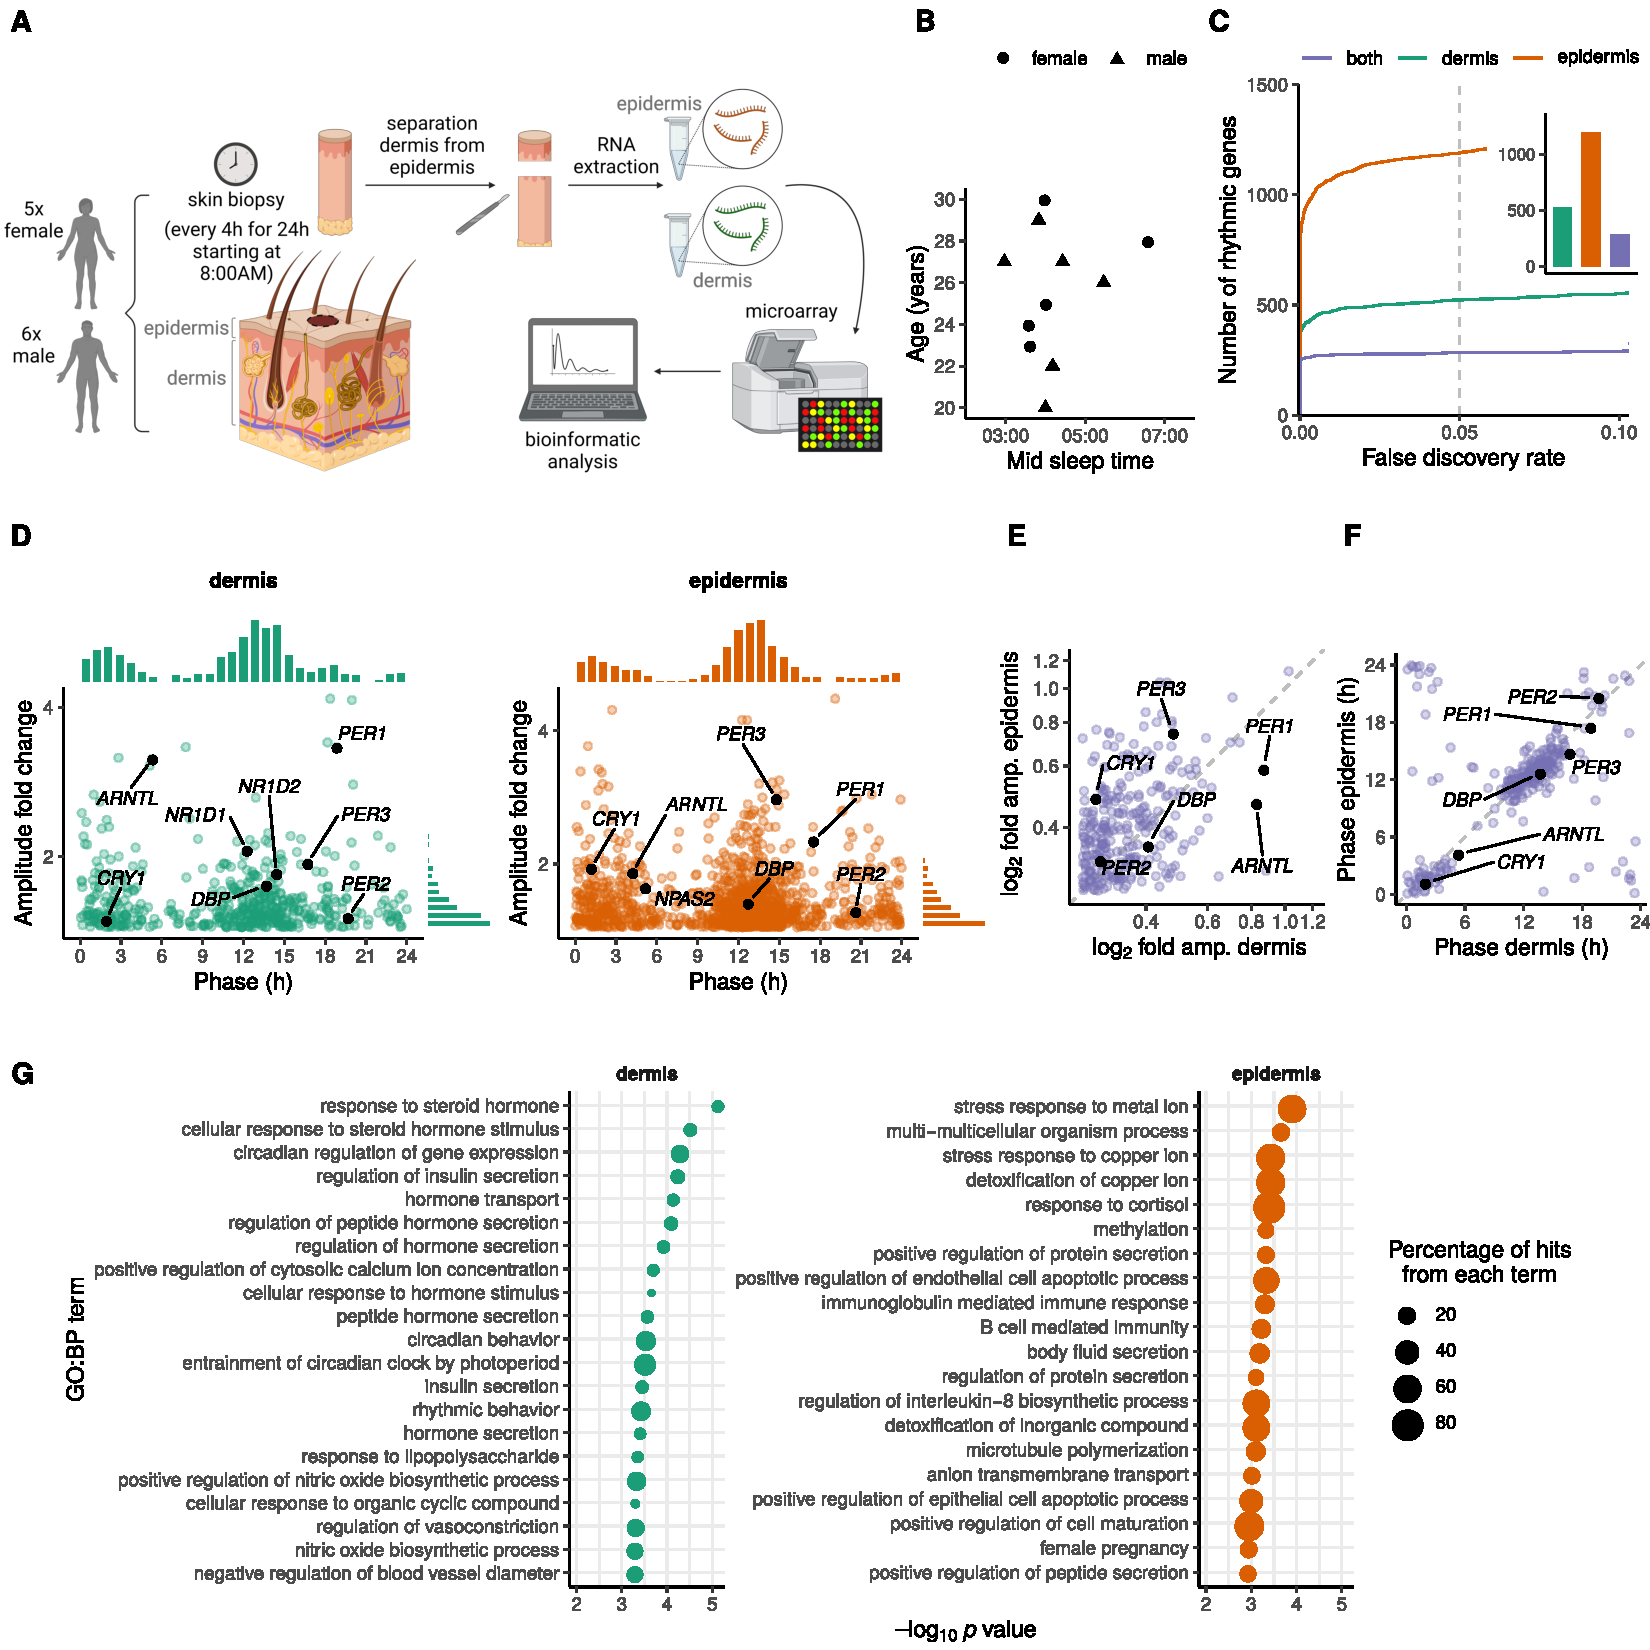
\includegraphics[scale=0.55]{./Figures/fig1_complete_ext.pdf}
		\caption{\textbf{Functional clocks in human dermis and epidermis. A.} Experimental setup: the dataset includes dermal and epidermal samples collected from the back of 11 healthy subjects (5 females, 6 males). Punch biopsies were collected every 4\,h for 24\,h starting at 8\,AM. Dermis and epidermis were separated and gene expression was analyzed using microarrays.\textbf{ B. }Composition of the study cohort by sex, age and mid sleep time. \textbf{C. }Number of circadian transcripts as a function of the false discovery rate (FDR). Rhythmic transcripts with respect to \textit{internal} time in dermis, epidermis or in both layers were determined by cosinor analysis (relative amplitude $>0.26$). For FDR$=0.05$ (inset), 523 transcripts were found to oscillate with a circadian period in dermis, 1191 in epidermis and 283 were common in both layers. \textbf{D. }Acrophase and amplitude distributions of the 24\,h cycling transcripts in human dermis (in green, left panel) and epidermis (orange, right panel) (FDR$<$ 0.05, relative amplitude $>$ 0.26). Each transcript is represented by a dot; clock genes are highlighted in black. \textbf{E. }Amplitude correlation of cycling transcripts in dermis \textit{and} epidermis. \textbf{F. }Phase correlation of cycling transcripts in dermis \textit{and} epidermis. \textbf{G.} Circadian GO enrichment analysis of the rhythmic genes in dermis (green) and epidermis (orange). The top 20 enriched biological processes (with a minimum gene set of 5 terms from each category) in each layer are shown. } %Thresholds: transform $\log(1+0.2)$ to ``biological words''.Maybe TODO: use internal time together with amp and phase fits to plot the gene expression curves in all 11 subjects. Then plot mean curve and determine amplitude from the population curve. Do the same but with wall time: Do amplitudes change? For which genes? \textcolor{red}{Think about DOSE with weights -- there was one skin term! Commented at end of 4th paragraph}. mingene set size=5}
		\label{fig:fig1}
	\end{center}
\end{figure*}

%as many external factors as possible, including chronotype

Population rhythm amplitudes have larger in the epidermis, but core clock genes are remarkably similar across layers. We observed a bimodal distribution of phases of all circadian dermal and epidermal genes, with peaks clustering at 2\,h and 13\,h after mid-sleep time on free nights (MSF\textsubscript{sc}, Figure \ref{fig:fig1}D and Supplementary Figure \ref{fig:suppfig2}A)\todo{in contrast to previous studies that have reported phases clustered at 8:00-9:00 and 20:00-21:00 \cite{Wu2018, Wu2020}).}. Despite the similarity of the distributions, amplitudes and phases of individual genes varied between skin layers: Among rhythmic genes common to the two layers, \todo{consistently use circadian genes or genes with circadian expression} epidermal circadian genes oscillate with a higher amplitude than those in the dermis among the differentially-rhythmic genes, with a trend in this direction among the circadian genes with similar rhythms (Figure \ref{fig:fig1}E). There was no systematic trend in the phase difference between common circadian genes in the two layers (Figure \ref{fig:fig1}F). The core clock genes were remarkably consistent (statistically indistinguishable) in amplitude and phase between the two layers (Supplementary Figure \ref{fig:suppfig2}B) with the exception of \textit{ARNTL} and \textit{PER3}, which had higher amplitudes in the dermis and epidermis, respectively. Note, NR1D1 and NR1D2 were rhythmic in both layers but with amplitudes just outside the amplitude cutoff in the epidermis.

(What is the conclusion out of this, I dont know :( )Dermal circadian genes were enriched in nitric-oxide metabolism, photoperiodic response, hormone-related terms and blood circulation, whereas the epidermis circadian transcriptome was enriched in terms related to the response to metals, regulation of fluid levels and wound healing, and response to cortisol (Figure \ref{fig:fig1}G). We also performed KEGG pathway enrichment analysis and found that infection-related and TNF signaling pathways appeared in dermis; on the other hand, the epidermal circadian genes was enriched in pathways associated to metabolism and phototransduction (Supplementary Figure \ref{fig:suppfig2}C). Morning-time genes were enriched for immune-related pathways together with phosphorylation and metabolic signaling, whereas the evening was marked by genes involved in carbohydrate, nitrogen and phenol metabolism (Supplementary Figure \ref{fig:suppfig2}D and E, as determined by phase set enrichment analysis (PSEA) \cite{Zhang2016}). \todo{is this phase, time after MSFsc?}

Population circadian rhythms are not affected by choice of time reference in this dataset. We repeated the above analysis without correcting the sample collection times for subject chronotypes using MSF\textsubscript{sc}. Interestingly, the circadian genes determined with respect to external time (Supplementary Figure \ref{fig:suppfig1}) did not deviate appreciably in number, amplitude or phase from the circadian genes (Figure \ref{fig:fig1}C,D,E,F) with respect to internal time, i.e, controlling for $\textrm{MSF}_\textrm{sc}$ did not affect rhythmicity analysis significantly in our dataset. \todo{for discussion -- This might be due to the range of MST, which is in the order of the sampling frequency, or because of additional sources of inter-individual variation.} 

In summary, we observed significant similarity in the circadian gene expression across these two adjacent skin layers complemented by some layer-specificity of circadian rhythms. 

%\textcolor{red}{\textbf{I've removed the correlation matrices from this figure}}.\\%To our surprise, we found no skin-related diseases when doing disease ontology enrichment analysis \cite{Yu2015}, but several pancreatic and cardiovascular-related conditions enriched in dermis (no significant diseases were enriched among the circadian epidermal transcriptome) (Figure \ref{fig:fig1}H).\\

%\scriptsize{\textcolor{red}{Are the most rhythmic genes in each layer related to a specific function? e.g. keratinization in epidermis? Also2: Do phases of genes correlate with the mid sleep time? I guess this question applies mostly to phases of ZeitZeiger genes}.}

%\footnotesize{\begin{itemize}
%	\item Human dermis and epidermis every 4h across a 24-h sampling period from 11 individuals (starting at 8\,AM)
%	\item \textbf{\underline{One}} single test (in the lines of \cite{Pelikan2021}) to identify rhythmic genes only in dermis versus only in epidermis versus in both layers.
%	\item Stable number of rhythmic genes independently of the exact FDR cutoff
%	\item Wall time corrected with mid sleep time $\rightarrow$ internal time: we think internal time should be taken into account if any evaluation of circadian phase of skin biomarkers is desired.
%		\begin{itemize}
%		\item Wall time and internal time give similar numbers of rhythmic genes $\rightarrow$ maybe because mid sleep time range is $\sim$ our sampling frequency?
%	\end{itemize}
%	\item Functional clocks present in human dermis and epidermis
%	\begin{itemize}
%		\item Careful with conclusions about tissues -- skin is very heterogeneous with various tissue types 
%		\item Clock amplitude and phase varies between skin layers: higher amplitude in epidermis (reason for more rhythmic genes?), dermis is later
%	\end{itemize}
%	\item Identification of clock-regulated transcriptome in human skin layers: we compared the circadian transcriptome of the two prominent skin layers in human skin, i.e. dermis and epidermis
%	\begin{itemize}
%		\item Amplitude and phases vary in similar fashion as do the clock genes
%		\item Bimodal phase distribution: two main peaks ast $\sim1$\,AM and $\sim1$\,PM \textcolor{red}{($\neq$Hogenesch!)}
%	\end{itemize}
%	\item GO terms (\textcolor{red}{KEGG better?}) all over the place \textbf{\textcolor{red}{-- slim them!}}, and not super significant:
%	\begin{itemize}
%		\item Dermis: rhythmic processes, hormone-related terms, blood vessel related processes \textcolor{red}{(viral, parasite and bacteria-related pathways)}
%		\item Epidermis: response to metals, immune-related terms, body fluid and protein secretion \textcolor{red}{(absorption, phototransduction, immune-related pathways)}
%	\end{itemize}	
%	\item Disease enrichment: related to cardiovascular disease, pancreatic conditions
%	\begin{itemize}
%		\item No skin-related conditions like psoriasis for example \textcolor{red}{-- move to the supplement?}
%	\end{itemize}	
%	\item \textcolor{red}{Are the most rhythmic genes in each tissue related to a specific function? e.g. keratinization in epidermis?}
%\end{itemize}}

%----------------------------------------------------------------------------------------
%----------------------------------------------------------------------------------------

\subsection*{Amplitudes and phases are subject-specific, while magnitudes are layer-specific}
The population (mean) circadian gene expression describes rhythmic gene expression at the level of the cohort. We next evaluated how variable circadian expression was within the cohort in relation to the variability across layers. In other words, how representative is the population gene expression of circadian expression in individuals. We fit linear-mixed-effect models \cite{Hoffman2016} followed by error propagation to obtain both the average circadian gene expression (fixed effects) and the variation across subjects and layer (random effects). For this analysis, we only considered the 1439 genes that showed rhythms at the population level in at least one layer. We characterized the variability in circadian parameters (magnitude (MESOR), amplitude and phase) of individual rhythmic genes across layers and subjects.

Magnitudes vary more across layers, and amplitudes and phases more across subjects. The error propagation analysis produced estimates of the variances of the circadian parameters across subjects and layers. We simultaneously characterized this variability in relation to the population circadian parameters using the coefficient of variation (CV). When the variability is viewed in absolute or relative terms, magnitude of circadian genes varied more across layers than across subjects, while amplitudes and phases were more variable across subjects than across layers (Figure \ref{fig:fig2}A). In order to better quantify the relative contribution of layer and subject to the circadian rhythm variability, we defined the fraction of variance explained by subject as $\sigma^2_\textrm{sub}/(\sigma^2_\textrm{sub} + \sigma^2_\textrm{lay})$. As seen in Figure \ref{fig:fig2}A, more genes were variable in amplitude and phase across subjects (have variance explained closer to one in Figure \ref{fig:fig2}B). However, specific genes were more or less subject (layer) variable in all three circadian parameters. \textit{PER1,2} and \textit{NR1D2} showed highly variable magnitudes and amplitudes across subjects, while positive regulators \textit{CLOCK}, \textit{BMAL} were very stable. The phases of core clock genes were also much more variable across subjects than across layers. \todo{plot vs CV in supplement.}

Amplitudes of rhythmic genes are more variable than phases. The percentage variation of amplitude exceeded variation of phases both across layers and across subjects (Figure \ref{fig:fig2}C). Genes with different population rhythms between layers (Figure \ref{fig:fig1}) showed high amplitude and phase variability across layers as expected. In agreement with population rhythm analysis, core clock genes had remarkably low variability in amplitude and phases across layers. However, the core clock genes were more phase variable across subjects, but with comparable amplitude variability across subjects and layers. \todo{is there more to unpack here? I cant see the grey points much at all.}

Amplitudes in the dermis of subjects differ more than in epidermis. We observed previously that epidermal population rhythms had greater amplitudes than dermal rhythms. In addition, when the variability was quantified in the two layers separately, amplitude variability in the dermis across subjects exceeded that in the epidermis. Nevertheless, magnitude and phase variability was consistent across the layers. 

%The total expression variance of a gene can be partitioned into the individual contributions of subject, sex, skin layer and time plus a residual variance. This simple model assumes that the effect of each component of variation on the gene expression is additive and independent of other components in the model. To relax this strict assumption, we also modeled interaction effects whereby the effect of time depended also on subject and skin layer. In the end, we quantified six sources of variability: 
%\begin{itemize}
%	\item inter-sex mean variation (variance in mean expression (magnitude) between males and females),
%	\item inter-layer mean variation (variance in magnitude only due to differences in skin layers),
%	\item inter-subject mean variation (variance in magnitude only due to differences between subjects), 
%	\item common circadian variation (variation in expression across time points common to all layers and subjects), 
%	\item inter-layer circadian variation (variance of the temporal profiles across the two layers) and
%	\item inter-subject circadian variation (variance of the temporal profiles across subjects).
%\end{itemize}
%With the number of subjects and samples per subject in this study, other two-way and multi-way interactions could not be determined using this data. 

\begin{figure*}[b!]
	\begin{center}
		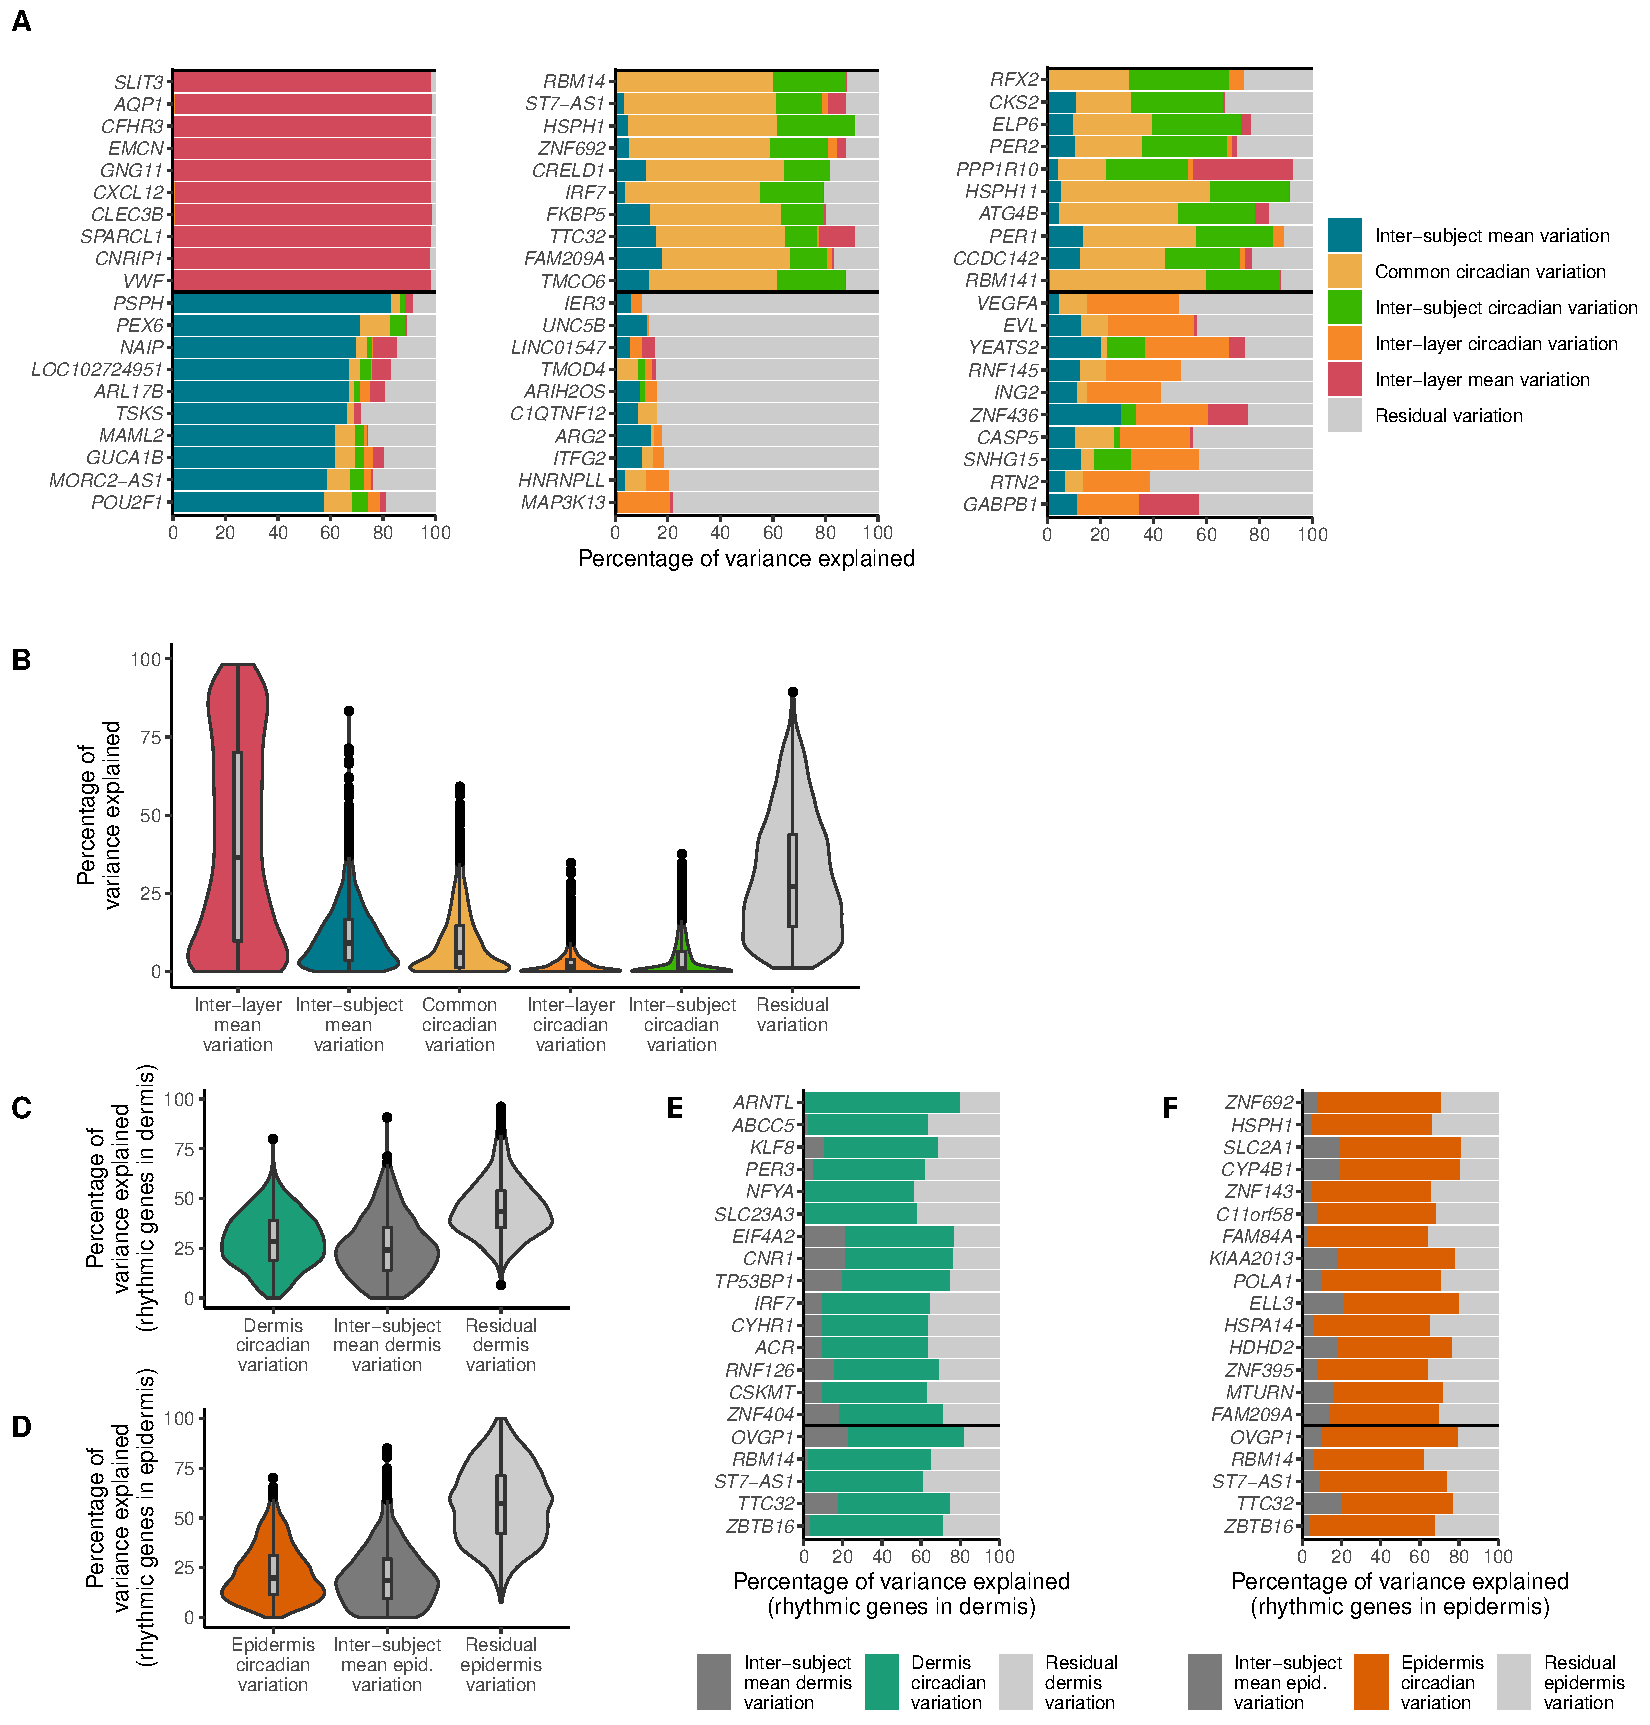
\includegraphics[width=\textwidth]{./Figures/fig2.pdf}
		%\caption{Identification of drivers of variation from the circadian transcriptome in human skin with variancePartition \cite{Hoffman2016}. A. Top 10 genes with highest variance in mean expression across layers (top left panel), across subjects (bottom left panel), across time (top middle panel) or with highest residual (unidentified) variation. The panels in the right show the top 10 genes with highest differences in circadian expression across subjects (i.e., rhythmic transcripts where rhythms seem to be subject-specific, top panel) or with highest differences in circadian expression across skin layers (i.e., rhythmic transcripts where rhythms seem to be dermis- or epidermis-specific, bottom panel). \textcolor{red}{Note how these results illustrate how variancePartition identifies genes where the majority of variation in mean expression is explained by a single variable, such as skin layer for \textit{SLIT3}, while variation in other genes is driven by multiple variables \textit{ZNF436}}. B. Quantification of the contribution of each meta-data variable to the variation in expression of each gene in a circadian transcriptome-wide trend, with the total contribution of each variable ranked in order from left to right (except the residual variation). \textcolor{red}{Should I make clear here what each metavariable means?}. To plot panels A and B, variancePartition was run with the $\sim~1400$ genes that are rhythmic in \textit{at least} one tissue and with external time as a meta-data variable (since internal time, a continuous variable, cannot be modeled as a random variable).}
		
		% \textcolor{red}{We previously argued that the common circadian variation is larger than the inter-subject/inter-layer circadian variation, and that this could be a reason to do ZeitZeiger on the whole dataset and not in dermis versus epidermis. If we are going to do ZeitZeiger on the whole dataset, should we maybe move panels C-F to the Supplement? They are still `informative' in the sense that they show that, taking all rhythmic genes in dermis (or epidermis), the largest source of variation in mean expression is variability across time and not subjects.}}
		%\label{fig:fig2}
	\end{center}
\end{figure*}

\begin{figure*}[!]
	\begin{center}
		%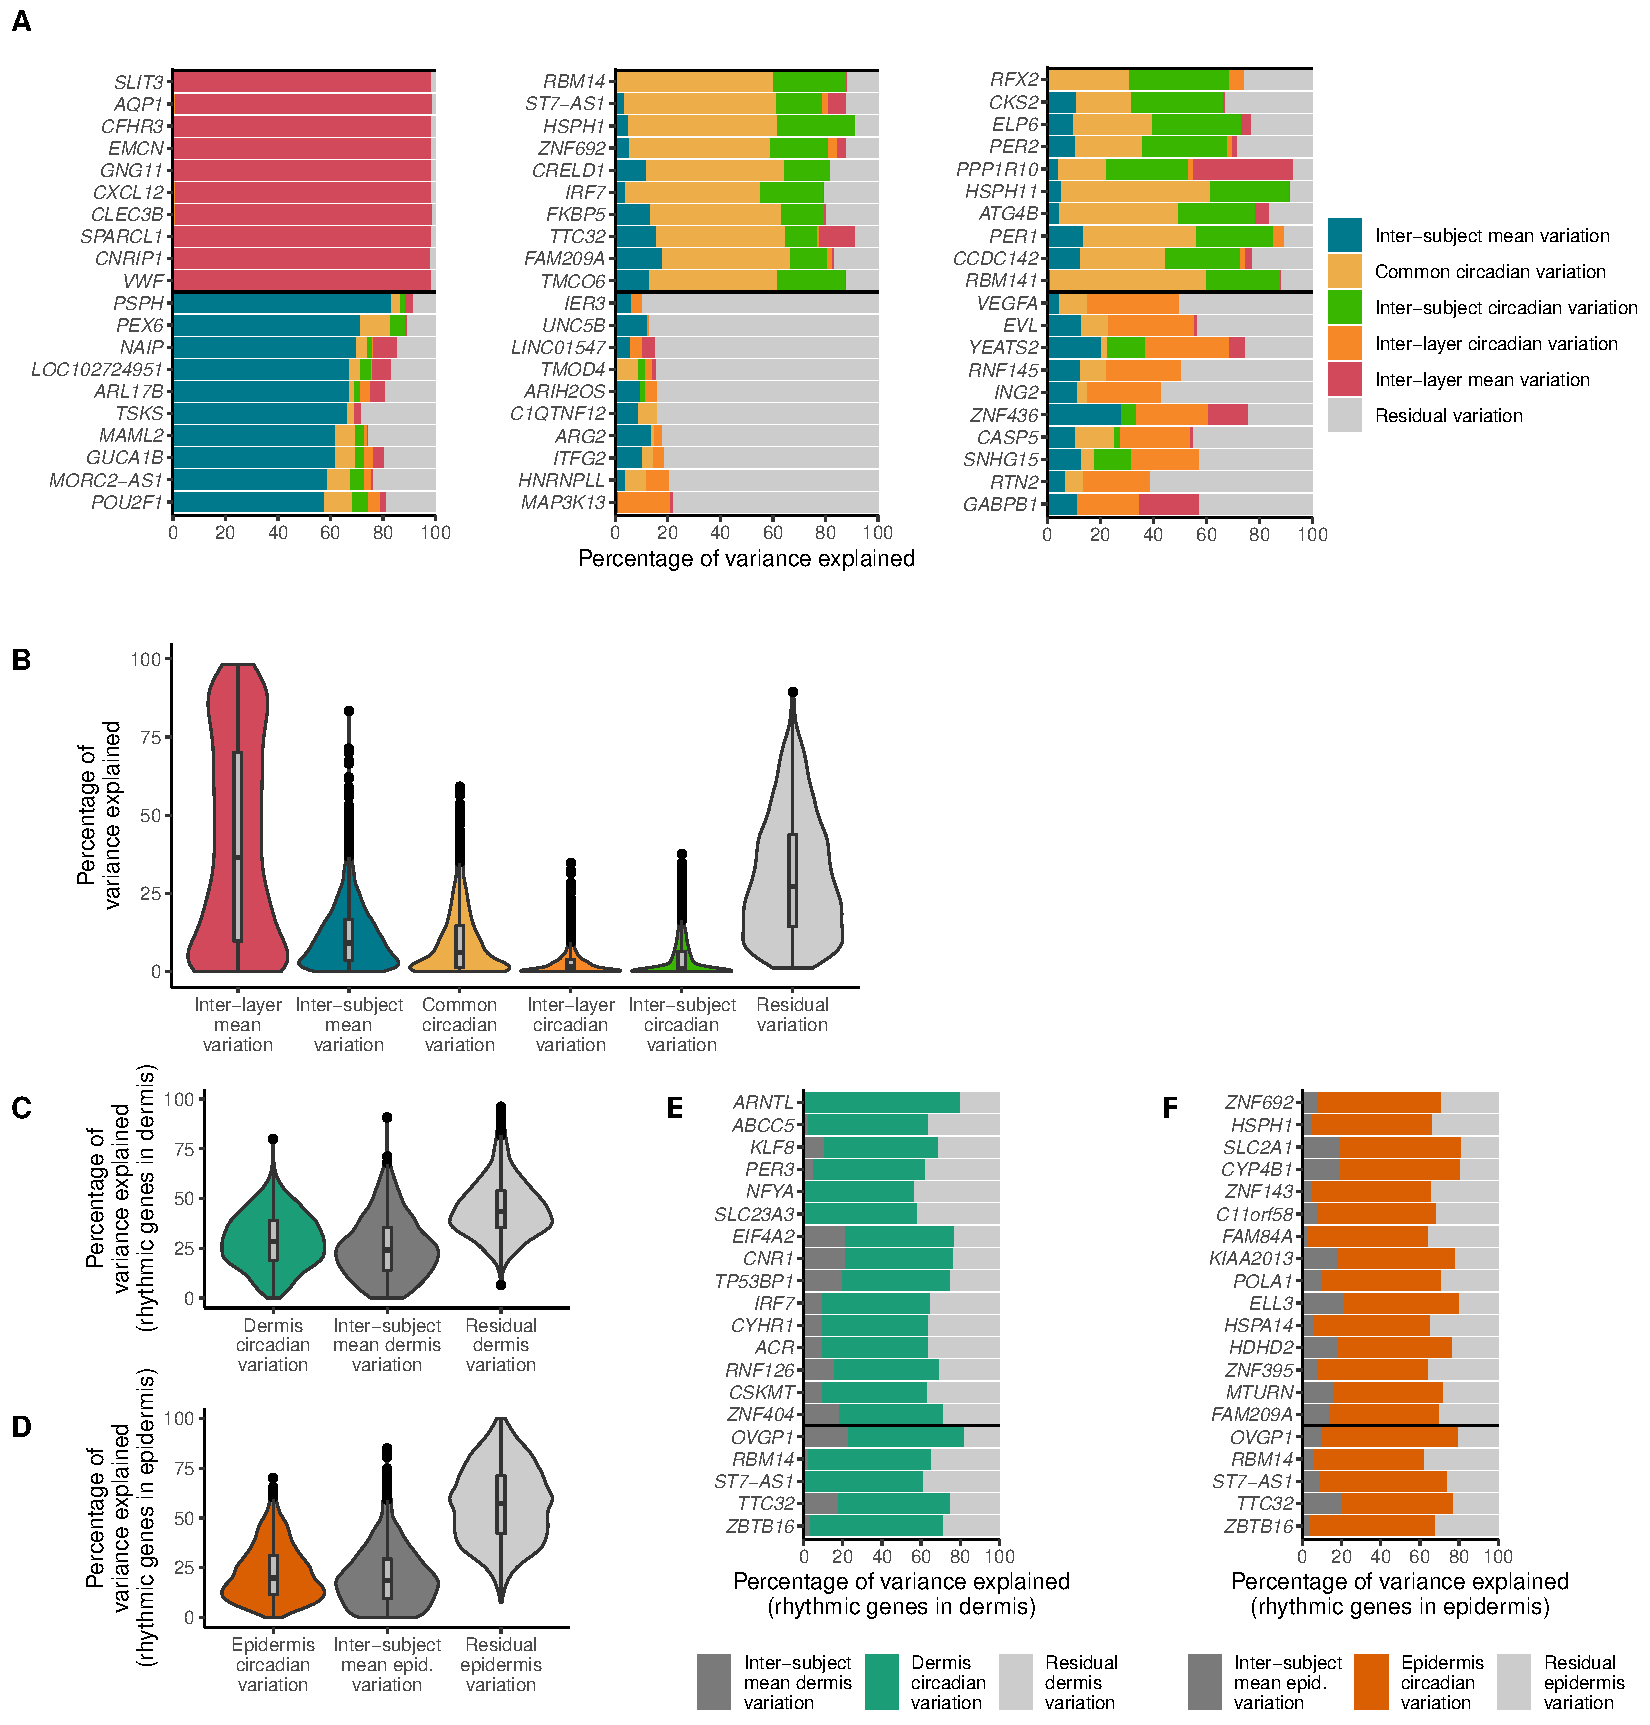
\includegraphics[scale=0.55]{./Figures/fig2.pdf}
		\caption{\textbf{Drivers of variation in the human circadian skin transcriptome identified with variancePartition. A.} Top 10 genes with highest variance in mean expression across layers (top left panel), across subjects (bottom left panel), across time (top middle panel) or with highest residual (unidentified) variation (bottom middle panel). The panels in the right show the top 10 genes with highest differences in circadian expression across subjects (i.e., rhythmic transcripts where rhythms seem to be subject-specific, top panel) or with highest differences in circadian expression across skin layers (i.e., rhythmic transcripts where rhythms seem to be layer-specific, bottom panel). \textbf{B.} Quantification of the contribution of each meta-data variable to the variation in expression of each gene in a circadian transcriptome-wide trend. To plot panels A and B, variancePartition was run with the $\sim1400$ genes that are rhythmic in \textit{at least} one layer and with external time as a meta-data variable. \textbf{C} and \textbf{D.} Contribution of each variable to variation in mean expression in the rhythmic genes in dermis (C) and epidermis (D). \textbf{E} and \textbf{F. } 20 genes with highest variation across time in dermis (E) and epidermis (F). Common time-varying genes across layers are depicted below the black line in panels E and F. variancePartition was run with the 523 rhythmic genes in dermis to plot panels C and E and with the 1191 rhythmic genes in epidermis to plot panels D and F.}
		
		% \textcolor{red}{We previously argued that the common circadian variation is larger than the inter-subject/inter-layer circadian variation, and that this could be a reason to do ZeitZeiger on the whole dataset and not in dermis versus epidermis. If we are going to do ZeitZeiger on the whole dataset, should we maybe move panels C-F to the Supplement? They are still `informative' in the sense that they show that, taking all rhythmic genes in dermis (or epidermis), the largest source of variation in mean expression is variability across time and not subjects.}}
		\label{fig:fig2}
	\end{center}
\end{figure*}
%Applying variancePartition to this data illustrates how the method can decouple biological variation into multiple components, including a residual variation which remains uncharacterized. Results from representative genes \todo{I think I like looking at the transcriptome wide result before we look at individual genes. Although I get what you are trying to do here.}show how variancePartition identifies genes where the majority of variation in mean expression is explained by a single variable such as skin layer (e.g., \textit{SLIT3}, Figure \ref{fig:fig2}A, left panel), while variation in other genes is driven by multiple variables (e.g. \textit{ZNF436}, Figure \ref{fig:fig2}A, right panel). These results, illustrated in a rhythmic skin transcriptome-wide manner, show that variation across skin layers represents the major source of magnitude variability and explains a median of 36.4\% of the variance from the rhythmic skin transcriptome (Figure \ref{fig:fig2}B). The median variance explained \todo{I dont think absolute values of the variance explained mean much with interaction terms, see variancePartition} by subject (9.1\%), common circadian variation (6.1\%), inter-layer circadian variation (1.4\%) and inter-subject circadian variation (0.9\%) are smaller, but with a high unidentified residual variation (27.3\%). Moreover, we found that neither chronotype nor sex contribute to variability in mean expression of rhythmic genes, as \texttt{variancePartition} attributed very little variance to these components ($<0.5$\%, \textcolor{red}{data not shown}). \\

%Of particular interest here were two things: firstly, the fact that subjects differ more strongly in mean expression than in circadian rhythms (compare blue violin plot to green violin plot from Figure \ref{fig:fig2}B). This means that although rhythms \textcolor{red}{(phases?)} of clock controlled genes are not very subject-dependent, their magnitudes are. Secondly, the observation that time variation does not seem to be layer- or subject-specific, since the inter-subject and inter-layer circadian variation appeared smaller than the common circadian variability. In other words, time alone can explain variation without being dependent on layer or subject in our cohort. This result, together with the almost nonexistent contribution of chronotype to variability and the findings from Supplementary Figure \ref{fig:suppfig1}, speaks for population sampling from skin providing a good estimation of circadian time, regardless of wall time or internal time. As negative and positive control of the variancePartition analyses, we checked that the time variation across 1000 non-rhythmic genes (FDR $>0.1$) was almost 0 (Supplementary Figure \ref{fig:suppfig3}A), while it represented the largest source of variation for clock genes (Supplementary Figure \ref{fig:suppfig3}B).\\ %Interestingly, we also found the residual variation to be high in previous human skin transcriptomic datasets \cite{GSE112660, GSE139300} that we reanalyzed (\textcolor{red}{data not shown}). 
%BA1: common circadian variation is strongest in our cohort so we expect these insights to translate across population.
%BA2: great that subject differs in mean a lot but not so much in circadian - I think it is not obvious/known that CCGs' magnitude varies quite a lot between subjects.

%\textcolor{red}{We performed \textcolor{red}{GO analysis in top 200 most variable genes from each category} and found that wound healing processes were enriched in those with high variation in mean expression across layers (\textcolor{red}{Supplementary Figure \ref{fig:suppfig3}C}). On the other hand, genes with highest circadian variation across skin layers (orange category from Figure \ref{fig:fig2}A) were enriched in pyruvate metabolism, phosphorylation and ATP generation processes (Supplementary Figure \ref{fig:suppfig3}D). As for the genes with highest (unidentified) residual variation, we found that they were enriched in processes related to cytoskeleton and stimuli detection (\textcolor{red}{Supplementary Figure \ref{fig:suppfig3}E}).\\}

%Performing \texttt{variancePartition} on the epidermal and dermal rhythmic genes separately hinted to what the drivers of variation in each layer separately are. Common circadian variation exceeded the inter-subject mean variation in gene expression in both skin layers (although the residual variation, in either case, was found to be larger than the other sources of variation, Figure \ref{fig:fig2}C, D). The clock genes \textit{ARNTL, PER3} were found among the top 20 common circadian varying genes in dermis, but not in epidermis (Figure \ref{fig:fig2}E). Some genes appeared to have a high variability across time in both layers: \textit{OVGP1, RBM13, TTC32} or \textit{ZBTB16} (shown in the bottom of Figure \ref{fig:fig2}E, below the black line). \\

%Of note, the variance in mean expression explained by skin layers represents also the highest source of variation in previously published skin circadian transcriptomic studies \cite{GSE112660, GSE139300}, and these also show high residual variability (\textcolor{red}{data not shown}). This suggests that the learnings from our dataset can be translated to larger populations. Interestingly, the quantification of variation in our data is robust to sampling frequency. This is, we found similar contributions of each biological source when the time series of rhythmic genes was made sparser by removing time points (\textcolor{red}{data not shown}). \\%\\
%\footnotesize{\begin{itemize}
	%\item We quantified inter-subject and inter-layer variability in mean and circadian expression of clock-controlled genes -- explain these these categories (e.g. genes with high ``inter-layer circadian variation'' refers to those genes that show different circadian rhythms between both layers, and genes with high ``inter-subject circadian variation'' refers to those rhythmic genes that vary between subjects)
%	\item Common circadian variation exceeds inter-subject and inter-layer circadian variation, thus we expect to find good time-telling genes sets even across layers \textcolor{red}{$\rightarrow$ reason to do ZeitZeiger on the whole dataset and not in dermis versus epidermis?}
	%\begin{itemize}
		%\item Inter-layer variation represents the biggest source of variability in mean expression. It is followed by mean inter-subject variation, which in turn exceeds common circadian variation. 
		%\item Big residual variation 
	%\end{itemize}	
	%\item Also Hogenesch's data shows big residual variation
	%\item Chronotype doesn't matter in skin: population sampling from skin provides a good estimation of circadian time (regardless of wall time or internal time)
	%\item Results independent of the number of datapoints taken (with 4 data points, similar variances -- data not shown)
%\end{itemize}}

%----------------------------------------------------------------------------------------
%----------------------------------------------------------------------------------------

\subsection*{Predictive biomarkers of internal time in human dermis and epidermis}
Finally, we assessed the viability of skin samples to be used for circadian phenotyping. When a fixed phase relationship between the skin clock and the central SCN clock is assumed, these biomarkers can serve as predictors of circadian phase of entrainment or chronotype. We identified biomarkers among genes expressed in either layer individually (as suggested by the layer-specificity) to predict \textit{internal} time from a single sample using \texttt{Zeitzeiger}.

%Details on the ZeitZeiger implementation and the main parameters it uses are provided in Materials and Methods. \\
A small set of population rhythmic genes accurately predict internal time. For an optimal parameter choice (Supplementary Figure \ref{fig:suppfig5})A\todo{(2 sparse principal components (SPC) and sparsity ($sumabsv$)=2))}, 8-12 rhythmic genes were sufficient to predict internal time with a median absolute error (MAE) of $\sim 0.96$\,h (Figure \ref{fig:fig3}A). The ability to infer internal time from a single sample can be seen in counter-clockwise arrangement of samples projected on the two SPCs (Figure \ref{fig:fig2}B). The biomarkers found in the two layers all exhibited robust population circadian rhythms (Supplementary Figure \ref{fig:suppfig5}C,D) with the exception of one gene \textit{FOCAD}, which was also rhythmic but with an amplitude below our cutoff. The genes chosen as biomarkers all showed particularly low variability in amplitude, magnitude and phase across subjects\todo{this is correct?} according to our analysis in the previous section (Supplementary Figure \ref{fig:suppfig5}B).

The biomarkers sets included layer-specific novel genes, but were depleted of core clock genes. Curiously, the biomarkers for internal time included only two canonical clock genes (\textit{PER3}, \textit{ARNTL}) and that too only in the dermal set. Moreover, the smaller biomarker set for the dermis shared only one circadian gene (\textit{OVGP1}) with the larger set for the epidermis. The biomarkers in the dermis consisted of genes that were circadian (at the population level) in both layers. However, the epidermal biomarker set included several genes that were rhythmic only in the epidermis (\textit{POLA1}, \textit{ROR1}, \textit{SOX5}, \textit{ZNF143}). These sets also overlapped poorly with previously published biomarkers for epidermis (\textit{ZBTB16}, \textit{FKBP5}, \cite{Wu2018}) and dermis (\textit{PER3}, \textit{ARNTL}, \cite{Wu2020}). \todo{ better in Discussion? These results imply that the circadian clock is well approximated by a two-dimensional oscillator. Moreover, this cyclical behavior in SPC space was observed for each individual subject (Supplementary Figure \ref{fig:suppfig5}C) suggesting that such an approach may be used to detect perturbations of the skin clock in humans}

%In both layers, a high proportion of the time-telling genes overlapped with the top 20 time-varying genes from VPA (highlighted in yellow in Figure\ref{fig:fig3}B). (\textit{OVGP1} was not only a highly time-varying gene, but also one of the top 20 genes that have different rhythms in epidermis compared to dermis (orange category from Figure \ref{fig:fig2}), and hence marked orange). In fact, on repeating VPA only on circadian biomarker genes, we found that common circadian variance represented the dominant driver of expression variation in both skin layers, while inter-subject variation  was minimal (\todo{does not match Supplementary Figure \ref{fig:suppfig5}B, also evident from the time series in Supplementary Figure \ref{fig:suppfig5}A}). In other words, biomarkers of circadian phase show little differences in mean expression (i.e., magnitude) across subjects and also possess strong circadian rhythms. 
\\



\begin{figure*}[t!]
	\begin{center}
		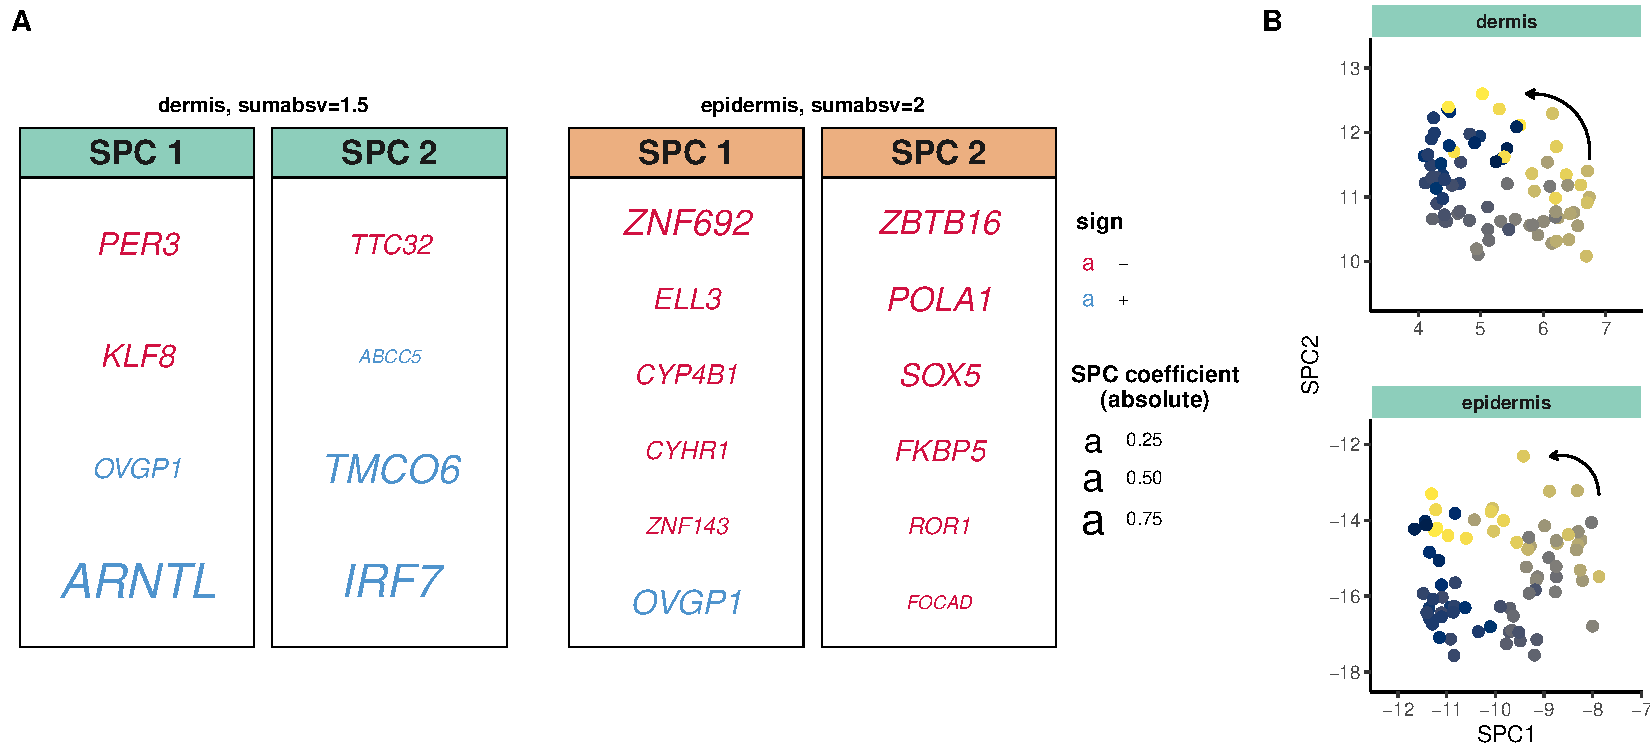
\includegraphics[width=\textwidth]{./Figures/fig3.pdf}
		\caption{\textbf{Identification of internal time-telling genes in human dermis and epidermis with \texttt{ZeitZeiger}. A. }Median absolute error of the internal-time prediction on cross-validation (see Materials and Methods for details) as a function of the two main parameters of ZeitZeiger, \texttt{sumabsv} and \texttt{nSPC}. \textbf{B. }Internal time predictors from human dermis (left panels) and epidermis (right panels) for \texttt{sumabsv}=2 and \texttt{nSPC}=2. Genes assigned to SPC1 or SPC2 as well as their coefficients are shown. Highlighted in yellow are genes that appeared in the top 20 most common circadian varying genes in the variancePartition analysis done in dermis and epidermis separately; in orange, genes that showed differential rhythms across layers (i.e., genes with high inter-layer circadian variation from the variancePartition analysis). \textbf{C. }Expression profiles of our cohort in dermis (left) and epidermis (right) represented in SPC space. Colors indicate the internal time of the subjects. ZeitZeiger was run with all $\sim11000$ expressed genes and separately for dermis and epidermis.}
		\label{fig:fig3}
	\end{center}
\end{figure*}

%To measure the accuracy of the prediction, \texttt{ZeitZeiger} uses the median absolute error (MAE): the lower this value, the better the prediction. Running \texttt{ZeitZeiger} in the whole set of $\sim11000$ skin-expressed genes (in either dermis \textit{or} epidermis) resulted in a minimum MAE of $\sim0.08$ for the software parameters \texttt{nSPC}=2 and \texttt{sumabsv}=3 (Supplementary Figure \ref{fig:suppfig4}A), with 38 genes needed for prediction (Supplementary Figure \ref{fig:suppfig4}B). On the other hand, running \texttt{ZeitZeiger} in each skin layer separately performed better, as seen by the lower MAE and the lower number of genes needed to predict internal time: 2 SPCs and \texttt{sumabsv}=2 resulted in a MAE of 0.04 in both layers (Figure \ref{fig:fig3}A) and a total of 15-25 genes needed for prediction (Figure \ref{fig:fig3}B, time series in Supplementary Figure \ref{fig:suppfig5}).\\ %\textcolor{red}{All three/two?} predictors performed comparably well, since the MAE did not decrease much after 2 sparse principal components (SPCs). However, the optimal value of \texttt{sumabsv} and, consequently, the number of genes used for prediction, differed in each approach.

Taken as a whole, our analysis indicates that either dermis or epidermis can be used for  phenotyping circadian phase using a small set of mostly skin-specific circadian genes.

%Our results indicate that dermis and epidermis time series data are well suited to extract time-telling genes, and that internal cross-validation performance is similar to that of previous studies \cite{Wu2018, Wu2020} \textcolor{red}{(I'm not sure if sfig7 and sfig8 really support this...)}. Moreover, integrated with prior published circadian skin transcriptomic studies, these results provide robustness, as some of the biomarker genes that we have found have already been described as skin phase-telling genes (\textit{ZBTB16, FKBP5, TRIM35, PER3, ARNTL}) \cite{Wu2018, Wu2020}. Moreover, although the common circadian variability exceeds the inter-subject and inter-layer circadian variation (Figure \ref{fig:fig2}A), and thus one could expect to find good time-telling gene sets even across layers, our results show that predicting internal phase in dermis and epidermis separately performs better than predicting internal time in skin as a whole. \\

\todo{Of note, ZeitZeiger was also used to predict external (wall) time. Although the accuracy of wall time predictors was comparable to those of internal time, the value of \texttt{sumabsv} was higher, thus resulting in a larger number of genes needed to predict wall time in both, skin as a whole, and in dermis versus epidermis separately (data not shown).}

%\footnotesize{\begin{itemize}
	%\item Zeitzeiger genes don't vary much in mean across subjects (useful) (data not shown)
	%\item ZeitZeiger genes in epidermis also found in Wu2018 \cite{Wu2018}: \textit{ZBTB16, FKBP5, TRIM35}
	%\item ZeitZeiger genes in dermis also found in Wu2020 \cite{Wu2020}: \textit{ZBTB16, PER3, ARNTL}
	%\item Is there a ``better'' marker for skin phase?
	%\item How good are the monocyte biomarkers in skin?
	%\item \textcolor{blue}{ZeitZeiger predicts phase... but can we come up with an amplitude predictor? Ratios of clock genes maybe?}
	%\item More time-telling genes if we use wall time, but since we want to predict \underline{internal} time it maybe makes more sense to use internal time
	%\item Candidate biomarkers that are robust to a different sample collection method?
	%\item Zeitzeiger genes are not any of the top 20 varying tissue-genes (vp full)
%\end{itemize}}


